%%%%%%%%%%%%%%%%%%%%%%%%%%%%%%%%%%%%%%%%%%%%%%%%%%%%%%%%%%%%%  
%
% SZABLON PRACY DYPLOMOWEJ
% WYMAGANIA ISE EITI PW
% AUTOR: Królik
% OPARTE NA SZABLONACH AUTORSTWA: Paszciora, Mastera & Kuchara
% 2011
% 
%%%%%%%%%%%%%%%%%%%%%%%%%%%%%%%%%%%%%%%%%%%%%%%%%%%%%%%%%%%%%
\author{Michał Haponiuk}
\title{Przeglądarka genomu}
\date{\today}

\documentclass[a4paper,12pt,oneside]{mwrep}  %bylo report
\usepackage[utf8]{inputenc} %ISO-8859-2 
\usepackage[polish]{babel} 
\usepackage{times} 
\usepackage[T1]{fontenc} 
\usepackage[MeX]{polski} 
\usepackage[pdftex]{color,graphicx} 
\usepackage{pdfpages} 
\usepackage{fancyhdr} %numery stron po zewnętrznej 
\usepackage{wrapfig}
\usepackage[bookmarks,unicode
			% odkomentowanie linijki poniżej usuwa kolorowe ramki w linkach
			%,colorlinks,citecolor=black,filecolor=black,linkcolor=black,urlcolor=black
			]{hyperref} 
\usepackage{titlesec} 
%\usepackage[dvi-ps]{graphicx}

%marginesy 
\usepackage[ bindingoffset = 1cm, hmargin = 2cm, vmargin = 2cm]{geometry} 
%interlinia 
\linespread{1.5} 

\widowpenalty=10000 % ostatni wierszrkapitu nie zostanie przeniesiony na następną stronę 
\clubpenalty=10000 % pierwszy wiersz akapitu nie będzie kończył strony (nie używam tego ustawienia)
\hbadness= 1450 %% zmniejsza liczę wyświetlanych ostrzeżeń (można zwiększyć, ale bez przesady)
\hfuzz = 0pt %% tekst może sterczeć ma marginesie na 1,5pt (ok. 0,5mm)

\clubpenalty=10000 %nie pozostawia sierot
\brokenpenalty=10000 %nie dzieli stron je»eli podziaª wyrazu
\sloppy %zakaz wydªu»ania lini

%wcięcia 
\setlength{\parindent}{1cm} 
\setcounter{secnumdepth}{2} %only sections and subsections are numbered 
\setcounter{tocdepth}{2} %table of contents shows up to three levels 



%eiti 
%rozdział 16pt, pogrubiona, kapitalki, interlinia 2 

\titleformat{\chapter}[hang] 
{\Large\bfseries}{\thechapter}{10pt}{\Large\bfseries} 
\titlespacing{\chapter}{0pt}{1em}{1em} 

%podrozdział 12pt, pogrubiona, kapitalki, il 2 
\titleformat{\section}[hang] 
{\normalfont\bf}{\thesection}{10pt}{\normalfont\large\bf} 
\titlespacing{\section}{0pt}{1em}{1em} 

%punkt 12pt, pogrubiona, il 2 
\titleformat{\subsection}[hang] 
{\normalfont\bf}{\thesubsection}{10pt}{\normalfont\large\bf} 
\titlespacing{\subsection}{0pt}{1em}{1em} 


%podpunkt 12pt, il 2 
\titleformat{\subsubsection}[hang] 
{\normalfont}{\thesubsubsection}{10pt}{\normalfont\bf} 
\titlespacing{\subsubsection}{0pt}{1em}{1em} 

\titleformat{\paragraph}[hang] 
{\normalfont}{\theparagraph}{10pt}{\normalfont\it} 
\titlespacing{\paragraph}{15pt}{1em}{1em} 

\renewcommand{\contentsname}{Spis treści} 
\renewcommand{\refname}{Bibliografia}


\begin{document} 

%%%%%%%%%%%%%%%%%%%%%%%%%%%%%%%%%%%%%%%
%STRONA TYTUŁOWA
%%%%%%%%%%%%%%%%%%%%%%%%%%%%%%%%%%%%%%%
\begin{titlepage} 

% Logo Politechniki Warszawskiej
\begin{figure*}
        
\includegraphics[width=2.5cm]{grafika/logo_pw} \hfill
        
\includegraphics[width=2.5cm]{grafika/logo_weiti}
\end{figure*}

\begin{center}

\LARGE{\textbf{POLITECHNIKA WARSZAWSKA}}\\
\Large{Wydział Elektroniki i Technik Informacyjnych}\\
\large{Instytut Informatyki}				%%% Instytut

\vfill

\vfill
\huge \textbf{Michał Haponiuk}\\  						 %%%Imie i nazwisko
\large{nr albumu: 249371}\\[1cm] 						 %%% numer albumu

\textsc{\Large Praca Dyplomowa Inżynierska}\\[1,5cm]     %%% rodzaj pracy

\huge \textbf{Przeglądarka genomu}\\[2cm] %%% Tytuł pracy

\vfill

\begin{flushright}
\large{Praca wykonana pod kierunkiem\\
dr~hab.~inż.~Robert~Nowak}\\[1cm] 
\end{flushright}


% Bottom of the page
\large{Warszawa, \today}

\end{center}
\end{titlepage} 

\pagestyle{empty}
\cleardoublepage 


\def\abstract{
   \vfil
   \begin{center}%
	   {\bfseries {\Large \abstractname}}%
   \end{center}
   \quotation
   }
   
   \def\endabstract{\par
   \endquotation
   }
   \thispagestyle{empty}

%%%%%%%%%%%%%%%%%%%%%%%%%%%%%%%%%%%%%%%%%%%%%%%%%%%%%%%%%%%%%   
% STRESZCZENIA
%%%%%%%%%%%%%%%%%%%%%%%%%%%%%%%%%%%%%%%%%%%%%%%%%%%%%%%%%%%%%
%\begin{abstract}
%
%
%	\begin{center}
%	{\bfseries Tytuł pracy}\\[0.3cm]
%	\end{center}
%	
%	
%Treść streszczenia	
%	
%
%\end{abstract}
%
%\renewcommand\abstractname{Abstract}
%\begin{abstract}
%	\begin{center}
%	{\bfseries Tytuł po angielsku}\\[0.3cm]
%	\end{center}
%	
%Treść streszczenia po angielsku
%	
%\end{abstract}
%
%\newpage	
%\thispagestyle{empty}
%\cleardoublepage 
%
%%%%%%%%%%%%%%%%%%%%%%%%%%%%%%%%%%%%%%%%%%%%%%%%%%%%%%%%%%%%%%  
% ZYCIORYS
%%%%%%%%%%%%%%%%%%%%%%%%%%%%%%%%%%%%%%%%%%%%%%%%%%%%%%%%%%%%%
%
%{


%\setlength{\parindent}{0pt}

%Imię i nazwisko: Imię Nazwisko\\
%Specjalność: Twoja Specjalność\\
%Data urodzenia: 31 lutego 2038\\
%Data rozpoczęcia studiów: 1 października 2007\\
%
%\vspace{4cm}
%\begin{center}
%\huge ŻYCIORYS
%\end{center}
%
%\vspace{2cm}
%Życiorys
%
%}
%\newpage	
%
%\cleardoublepage 


%%%%%%%%%%%%%%%%%%%%%%%%%%%%%%%%%%%%%%%%%%%%%%%%%%%%%%%%%%%%%  
% SPIS TRESCI
%%%%%%%%%%%%%%%%%%%%%%%%%%%%%%%%%%%%%%%%%%%%%%%%%%%%%%%%%%%%%
\tableofcontents

\newpage



%\cleardoublepage
\pagestyle{plain}

%%%%%%%%%%%%%%%%%%%%%%%%%%%%%%%%%%%%%%%%%%%%%%%%%%%%%%%%%%%%%  
% PRACA WLASCIWA
%%%%%%%%%%%%%%%%%%%%%%%%%%%%%%%%%%%%%%%%%%%%%%%%%%%%%%%%%%%%%
\chapter{Przeglądarki genomów}

Bioinformatyka jako dziedzina nauki łączy w~sobie informatykę i~matematykę w~celu przetwarzania danych biologicznych. Szybki rozwój genomiki i~biologii molekularnej doprowadził do powstania ogromnej ilości informacji. Eksperymenty biologiczne zaczęły generować ogromne ilości danych, które okazały się trudne do przechowywania i~,,ręcznego'' przetwarzania. Biolodzy w~swojej pracy byli zmuszeni do skorzystania z~komputerów i~informatyki na etapach gromadzenia, wydobywania oraz przetwarzania informacji zawartych w DNA\footnote{Kwas deoksyrybonukleinowy} (rys.\ref{model-dna}), RNA\footnote{Kwas rybonukleinowy} i~białkach.

\begin{figure}[!h]
\centering

\includegraphics[width=0.83\textwidth]{grafika/DNA2}
%zdjecie z http://wideshut.co.uk/wp-content/uploads/2013/07/DNA.jpg
%zdjecie https://forensicdnaconsulting.files.wordpress.com/2013/07/canstockphoto2267476.jpg
\caption{Prosty model DNA.}
\label{model-dna}
\end{figure}

Matematyka wraz z~informatyką dostarczają niezbędnych narzędzi do rozwiązywania problemów związanych z~biologią. Pociąga to za sobą powstanie i~zarządzanie zaawansowanymi bazami danych, w~których mogą być przechowywane i~efektywnie eksplorowane dane biologiczne. Kolejną ważną częścią bioinformatyki jest aspekt obliczeniowy, czyli wykorzystanie komputerów do przetwarzania danych. Matematyka pozwala przy pomocy równań zamodelować pewne zjawiska, ale przede wszystkim do skonstruowania rozwiązań potrzebne są efektywne algorytmy i programy komputerowe.

Przeglądarki genomów są narzędziem, którym posługuje się bioinformatyka sekwencji. Dzięki nim możliwe jest katalogowanie informacji biologicznych, przeszukiwanie baz danych sekwencji, porównywanie genomów i~sekwencjonowanie. Otwarte podejście do stosowania narzędzi bioinformatycznych znacząco skraca czas planowania i przeprowadzania eksperymentów oraz oszczędza pieniądze.

Obecne przeglądarki są w~formie graficznych interfejsów, wyświetlających dane genomów z~biologicznych baz danych wraz z~adnotacjami. Umożliwiają naukowcom wizualizacje całych genomów z dodatkowymi informacjami pozyskiwanymi zwykle z wielu źródeł\footnote{Dane porównawcze (drzewa filogenetyczne, zmienności), laboratoryjne badania analityczne (sekwencje, skany), odnośniki do innych baz, przetworzone dane laboratoryjne.}. Różnią się one od zwykłych biologicznych baz danych, gdyż dane prezentowane są w~graficznym formacie ze współrzędnymi genomów naniesionymi na oś. Rysunek \ref{przykladowa-przegladarka-genomu} ilustruje typową wizualizację genomu.

\begin{figure}[!h]
\centering
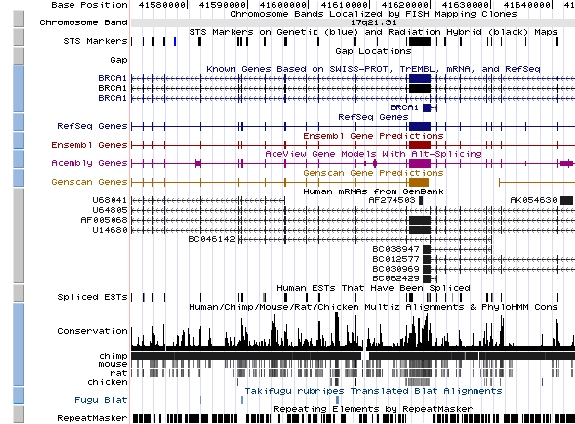
\includegraphics[width=0.75\textwidth]{grafika/browsershot_ucsc}
%zdjecie z https://genomics.soe.ucsc.edu/research/browser_overview
\caption{Fragment typowej wizualizacji genomu.}
\label{przykladowa-przegladarka-genomu}
\end{figure}

\section{Mapowanie genomów}
Nieodzownym elementem tworzenia przeglądarki genomów jest sporządzenie map przedstawiających położenie poszczególnych genów na chromosomie. Wyróżnia się \emph{mapy genetyczne}, określające odległości pomiędzy charakterystycznymi sekwencjami - markerami, oraz \emph{mapy fizyczne}, przedstawiające rzeczywistą pozycję poszczególnych genów. Informacje zawarte w mapach fizycznych i~genetycznych uzupełniają się nawzajem i~stanowią podstawę dalszych badań nad organizacją i~budową chromosomów. 

\subsection{Mapy genetyczne}
Mapy genetyczne na podstawie analizy sprzężeń genetycznych pozwalają ustalić rozmieszczenie genów i~innych charakterystycznych sekwencji (markerów) w genomie oraz określają odległości genetyczne pomiędzy nimi. Jednostką w tych mapach jest centymorgan\footnote{Jeden cM  to taka odległość pomiędzy dwoma loci, że szansa na ich rozdzielenie w procesie rekombinacji genetycznej w ciągu jednego pokolenia (podczas jednorazowego wydarzenia, np. crossing-over) wynosi 1\%.Centymorgany nie odzwierciedlają bezwzględnej odległości pomiędzy obszarami chromosomu zajmowanymi przez gen, ponieważ częstość rekombinacji jest różna w różnych rejonach chromosomów, na różnych chromosomach oraz w różnych organizmach.} (cM).

\subsection{Mapy fizyczne}
Mapy fizyczne wykorzystują techniki biologii molekularnej do bezpośredniej lokalizacji różnych typów sekwencji DNA w genomie. Stosowaną jednostką są tu pary zasad\footnote{Para zasad to dwie komplementarne zasady nukleotydów dwóch różnych nici kwasu nukleinowego, połączone wiązaniem wodorowym.} (pz). Tablica~\ref{lancuchy_DNA} przedstawia dwa komplementarne łańcuchy, oba mające długość 15 pz.
\begin{table}[!hb]
	\begin{center}
		\begin{tabular}{c|c|c|c|c|c|c|c|c|c|c|c|c|c|c|c|c|c|c|}\cline{2-16}\emph{Łańcuch 1}&
		\verb|A|&\verb|T|&\verb|C|&\verb|G|&\verb|A|&\verb|T|&\verb|T|&\verb|G|&\verb|A|&\verb|G|&\verb|C|&\verb|T|&\verb|C|&\verb|T|&\verb|A|\\ \cline{2-16}
		\emph{Łańcuch 2} &\verb|T|&\verb|A|&\verb|G|&\verb|C|&\verb|T|&\verb|A|&\verb|A|&\verb|C|&\verb|T|&\verb|C|&\verb|G|&\verb|A|&\verb|G|&\verb|A|&\verb|T|\\ \cline{2-16}
		\end{tabular}
	\end{center}
\caption{Komplementarność zasad w przykładowym łańcuchu DNA.}
\label{lancuchy_DNA}
\end{table}

\section{Historia}
Początki bioinformatyki sięgają lat osiemdziesiątych, kiedy to utworzono w~Stanach Zjednoczonych bazę danych zwaną \emph{GenBankiem}. Wraz z~coraz częstszymi badaniami różnych organizmów i~sekwencjonowaniem ich przez badaczy, Amerykański Departament Energii zdecydował się na opracowanie ww. programu, aby zbierać i sekwencjonować krótkie odcinki DNA. 

Początkowo użytkownicy wprowadzali sekwencje DNA do systemu używając specjalnych klawiatur posiadających jedynie cztery klawisze - A, C, T oraz G. Z~biegiem czasu opracowano specjalne protokoły przekazywania danych przyspieszające cały proces. Naukowcy mogli zadzwonić do \emph{GenBanku} i~używając komputera byli w stanie bezpośrednio wprowadzić dane o kolejnych fragmentach genomu do bazy (rys.\ref{historia-przeplywu-danych-sekwencji}). Rozwój technologi internetowych diametralnie zmienił sposób przekazywania informacji pomiędzy ośrodkami naukowymi. Po utworzeniu serwisu WWW, uczeni z całego świata otrzymali bezpłatny dostęp do zgromadzonych danych.

Zarząd \emph{GenBanku} przeniesiono do NCBI\footnote{National Center for Biotechnology Information} w~National Insitutes of~Health. Gdy w~1990~roku oficjalnie wystartował Projekt Poznania Ludzkiego Genomu, ilość informacji napływająca do \emph{GenBanku} rosła w tempie wykładniczym. Wraz z~opracowaniem wydajnych metod sekwencjonowania wykorzystujących komputery, automatyczne sekwencjonery i zagadnienia robotyki, proces gromadzenia danych niesamowicie przyspieszył.

Równolegle prywatne firmy również zajęły się podobnymi badaniami tworząc własne ogromne bazy danych. Obecnie największe korporacje są w stanie odczytać w ciągu jednego dnia zapis genetyczny liczący około 20 milionów par zasad DNA. Ilość danych jaką uzyskano z pełnej sekwencji genomu ludzkiego to ponad 50~TB\footnote{Taka ilość informacji zajęłaby 80 tys. płyt kompaktowych.}
\begin{figure}[!h]
\centering
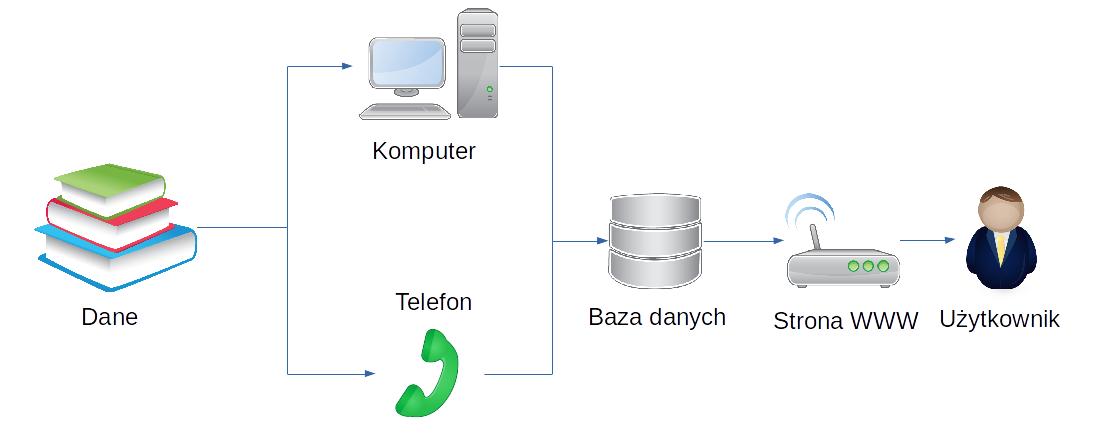
\includegraphics[width=0.9\textwidth]{grafika/historia.png}
\caption{Historyczny schemat przepływu informacji o sekwencjach.}
\label{historia-przeplywu-danych-sekwencji}
\end{figure}

\section{Oprogramowanie i narzędzia}
Spektrum oprogramowania dostępnego dla bioinformatyki jest bardzo szerokie. Rozpoczyna się od prostych narzędzi z~interfejsem terminalowym, a~kończy na usługach internetowych i~złożonych programach z~możliwościami rozbudowanej interakcji z~użytkownikiem.

Znaczna część narzędzi jest dostępna w formie darmowej lub otwartego oprogramowania. Następstwem zapotrzebowania na nowe algorytmy służącego do analizy był dynamiczny rozwój darmowych programów. Dzięki ideologii otwartego kodu źródłowego, grupy badawcze z całego świata mogą przyczynić się do tworzenia coraz to lepszych rozwiązań. Istotną zaletą darmowego oprogramowania jest tworzenie pewnych standardów i~integrowanie bioinformatycznych danych.

\subsection{Bazy danych}
Bazy danych używane w przeglądarkach genomów zwykle są ogromnymi zbiorami informacji, w~większości składającymi się z~danych sekwencji z~grupy kwasów nukleinowych. Z~powodu, że~są konieczne przy badaniach naukowych tworzenie ich jest jednym z najistotniejszych zagadnień w~bioinformatyce. Dane przechowywane w biologicznych bazach nie są niezmienne i~ostateczne. Wszystkie sekwencje są wynikiem badań o~jakiejś dokładności. Okazuje się, że czasami dane zgromadzone w bazach zawierają jednak nieprawidłowości.

Możliwość szybkiego i~precyzyjnego wyszukiwania pożądanych informacji jest jedną z~ważniejszych cech biologicznych baz danych. Najczęściej użytkownik oprócz obróbki danych ma również możliwość połączenia się przez internet z~innymi bazami. Charakteryzują się zazwyczaj, także małą redundancją danych. By ułatwić pracę, uczeni często mają możliwość wyboru sposobu wyświetlania wyszukanych danych oraz wydruku bądź zapisu ich.

Pierwsze bazy danych zazwyczaj budowali biolodzy molekularni i biochemicy. W dzisiejszych czasach zwraca się uwagę, aby były one czytelne nie tylko dla specjalistów, ale i dla badaczy z nauk pokrewnych biologii.

\subsection{Usługi internetowe}
Dla wielu zastosowań bioinformatycznych zostały opracowane interfejsy wykorzystujące protokoły SOAP\footnote{Simple Object Access Protocol - protokół komunikacyjny, korzystający z~XML do kodowania wywołań.} i REST\footnote{Representational State Transfer - styl architektury oprogramowania wywiedziony z doświadczeń przy pisaniu specyfikacji protokołu HTTP dla systemów rozproszonych, wykorzystuje m.in. jednorodny interfejs oraz bezstanową komunikację.}. Dzięki takim rozwiązaniom, aplikacja działająca w~jednej części świata jest w~stanie używać algorytmów, danych i~zasobów obliczeniowych serwerów podpiętych do sieci w~innych częściach świata. Największe udogodnienia wynikają z~faktu, że użytkownicy końcowi nie muszą zajmować się utrzymywaniem baz danych oraz oprogramowaniem. Usługi bioinformatyczne zostały podzielone na trzy podstawowe filary: dotyczące poszukiwania sekwencji, wielokrotnego przyrównywania sekwencji oraz analizy biologicznych sekwencji. Podział nastąpił z inicjatywy Europejskiego Instytutu Informatyki (EBI).

\section{Najpopularniejsze przeglądarki}
\subsection{Dostęp}
Na rynku obecnie dostępne jest wiele przeglądarek. Dzięki ogólnoświatowej sieci komputerowej są szeroko używane przez badaczy. Nie zawsze jednak możemy używać przeglądarek \emph{online}. Możemy nie chcieć udostępniać danych na zewnątrz, albo możemy posiadać ich za dużo by przesłać je na serwer z~innego krańca świata. Lekarstwem na ten problem są przeglądarki \emph{offline} wyświetlające dane z dysku, ale pobierające kontekst opisu genomu ze zdalnego serwera DAS\footnote{\emph{Distributed Annotation System} to protokół wymiany danych stworzony w celu publikowania oraz integracji danych biologicznych, w systemie rozproszonym.}.
\subsection{Architektura}
Różnią się niekiedy architekturą. Jedne są scentralizowane, inne stawiają na rozproszony system przechowywania baz danych. Oba podejścia charakteryzują się wadami i~zaletami, w~zależności od rozpatrywanego punktu widzenia. Projekty zaprzęgające dużą część społeczności naukowej wymagają wysiłku od dużej liczby osób, często powodując wygasanie entuzjazmu w~pracy oraz wymaga praktycznie ciągłej aktualizacji. Specjalizowane bazy danych z~silną kuratelą %np.Swissprot
zmagają się niekiedy z~problemami finansowymi. Sprawowanie ciągłej kontroli nad systemem również opóźnia dostęp do danych. Praktyka pokazuje, że~tylko nieliczne bazy danych rozwijające się w~zamkniętych społecznościach mają szansę dobrze funkcjonować, co rzutuje na popularność użytkowania przeglądarek genomów. Scentralizowane archiwa %(np.GenBank)
posiadają niekiedy kiepskie, niespójne albo wręcz żadne adnotacje\footnote{Adnotacja jest daną powiązaną z jakimś elementem (np.sekwencją), dostarczającą nowych informacji na temat tego elementu.} genomów.

\subsection{Przykłady}
\begin{itemize}
\item \href{https://genome.ucsc.edu}{\emph{UCSC browser}} \label{UCSC}
autorstwa Jima Kenta, napisana w~większości w~języku~C w~2000~roku. Udostępniana darmowo dla akademickich zastosowań. Dla komercyjnych zastosowań wymagana licencja \emph{Kent Informatics}.
\item \href{http://gbrowse.org}{\emph{Gbrowse}} - \label{Gbrowse}
największa część kodu to Perl, z czasem coraz więcej java-scriptu. Prace rozpoczęto w~2002 roku, funkcjonuje na licencji \emph{PERL artistic license}.
\item \href{http://www.ensembl.org}{\emph{ENSEMBL}} \label{ENSEMBL}
- funkcjonuje na licencji Apache, dopuszczającej użycie kodu źródłowego zarówno na potrzeby wolnego oprogramowania, jak i zamkniętego oprogramowania komercyjnego. Znaczna część kodu napisana w Perlu, schemat bazy danych w MySQl.
\item \href{http://bioviz.org/igb/index.html}{\emph{Integrated Genome Browser}} \label{IGB}
 - projekt rozpoczęty przez firmę \emph{Affymetrix}, jednak porzucony przez nią i rozwijany w środowisku akademickim. Przeglądarka napisana w Javie, obecnie na prawach Academic free license.
\end{itemize}

\chapter{Projekt i implementacja}
Aplikacje wykorzystywane do analizy danych genetycznych, korzystają zazwyczaj z~ogromnych woluminów i złożonych algorytmów. Wysoka wydajność, elastyczność oraz interfejs użytkownika z~wykorzystaniem przeglądarki internetowej to cechy aplikacji, które można osiągnąć łącząc ze sobą kilka języków programowania.
\cite{bioweb}

Dane genetyczne przedstawiane są typowo w postaci zbiorów łańcuchów znaków, gdzie każdy ciąg jest sekwencją symboli z~danego alfabetu. Reprezentacja łańcuchowa zwana pierwszorzędową (rys.\ref{rzedowe-struktury-bialek}a), odzwierciedla fakt, że~cząsteczki przechowujące informacje genetyczne (DNA i~RNA) są biopolimerami\footnote{Polimer występujący naturalnie w organizmach żywych, produkowany przez nie.} nukleotydów\footnote{Podstawowy składnik strukturalny kwasów nukleinowych.}, podczas gdy proteiny\footnote{Białka, wielocząsteczkowe biopolimery.} są łańcuchami polipeptydowymi\footnote{Łańcuchy cząstek aminokwasów połączonych wiązaniem peptydowym, po uzyskaniu odpowiedniej struktury przestrzennej może stać się funkcjonalnym białkiem.}. By zrozumieć wzajemne relacje pomiędzy nukleotydami a aminokwasami należy przyjrzeć się drugo, trzecio oraz czwartorzędowym strukturom. Struktura drugorzędowa (rys.\ref{rzedowe-struktury-bialek}b) obejmuje wiązania wodorowe pomiędzy nukleotydami DNA i~RNA oraz wiązania wodorowe pomiędzy peptydami w proteinach, określające przestrzenne ułożenie cząstek. Trzeciorzędowa struktura (rys.\ref{rzedowe-struktury-bialek}c) określa położenie atomów w trójwymiarowej przestrzeni, natomiast czwartorzędowa (rys.\ref{rzedowe-struktury-bialek}d) opisuje wyższy stopień organizacji wyjaśniający sposób łączenia się struktur trzeciorzędowych.
\cite{bioweb, pl-wiki-biopolimer, pl-wiki-nukl, pl-wiki-bialka, pl-wiki-2nd-struct, e-biotech-bialka}

Wzbogacając model o~informacje opisujące zależności pomiędzy ciągami a podciągami, możliwa jest analiza podobieństwa z wielu peryspektyw. Ponadto, dane te uzupełnione o~opisy czytelne dla człowieka ułatwiają zrozumienie znaczeń sekwencji oraz funkcji jakie pełnią.
\cite{bioweb}
\begin{figure}[!h]
\centering
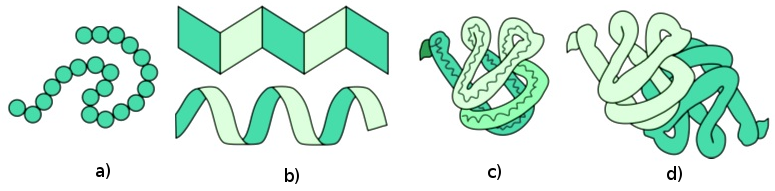
\includegraphics[width=1\textwidth]{grafika/struktury_bialek.png}
\caption{Rzędowość struktury białek: pierwszorzędowa (a), drugorzędowa (b), trzeciorzędowa (c), czwartorzędowa (d).}
\label{rzedowe-struktury-bialek}
\end{figure}

Charakterystyczną cechą programów komputerowych korzystających z~danych genetycznych jest konieczność analizy ogromnych zbiorów danych za pomocą skomplikowanych algorytmów, co oznacza, że~wysoka wydajność jest kluczowa. Różnorodność systemów i użytkowników sprawia, że przenośność oprogramowania jest równie ważna. Badacze preferują korzystanie z~aktualizowanych automatycznie, graficznych interfejsów użytkownika dostępnych z~poziomu przeglądarek internetowych.
\cite{bioweb}

Inżynierowie starają się rozwiązywać występujące na globie praktyczne problemy. Naukowcy próbujący opisywać i~wyjaśniać świat są coraz bardziej zaangażowani w rozwój oprogramowania. W~celu przyspieszenia procesu tworzenia aplikacji oraz uniknięcia typowych błędów, badacze powinni korzystać ze zbioru metod, technik i technologii, którymi dysponuje dziedzina nauki nazywana inżynierią oprogramowania. Dzięki sprawdzonym praktykom możliwe staję się projektowanie systemów spełniających stawiane im wymagania.
\cite{bioweb, inz-opr-k.sacha}

\section{Architektura}
Aplikacja została zrealizowana w trójwarstwowej architekturze, gdzie warstwa prezentacji, przetwarzania oraz danych są wyraźnie odseparowane od siebie. Użycie wielowarstwowego modelu sprawia, że programy komputerowe są przenośne i wielorazowego użytku. Idea ta odzwierciedla fakt, że poszczególne moduły pełnią różne role w systemie. Warstwy pomagają oddzielić od siebie różne podsystemy, ułatwiając jednocześnie utrzymanie dobrze zorganizowanego, czytelnego kodu.
\cite{bioweb}

Oprogramowanie zostało zbudowane w oparciu o swobodnie dostępny framework \mbox{\emph{bioweb}} przystosowany do analizy danych genetycznych używający C++, Python (django), \mbox{JavaScript} (AngularJS) i kilku innych bibliotek. \emph{Bioweb} został niejednokrotnie użyty do tworzenia aplikacji przetwarzających dane genetyczne skracając czas i koszty pracy do minimum.
\cite{bioweb}

Podczas projektowania aplikacji trójwarstwowej należy rozpatrzeć cztery możliwe modele: desktopowy (rys.\ref{klient-serwer}a), z~serwerem bazodanowym (rys.\ref{klient-serwer}b), z cienkim klientem (rys.\ref{klient-serwer}c), oraz aplikację webową(rys.\ref{klient-serwer}d). Aplikacja desktopowa nie jest dobrym rozwiązaniem w projektowanym systemie, ponieważ nie zapewnia dostępu dla wielu użytkowników. Jedynie osoba korzystająca w~danej chwili ze stacji roboczej mogłaby używać systemu. Z~powodu braku scentralizowanego serwera bazodanowego ciężkim zadaniem stałoby się umożliwienie współpracy zespołom naukowym. Z~racji łatwo dostępnej ogólnoświatowej sieci komputerowej użytkowanie systemów w~trybie offline staje się bardzo rzadkie. Bazy danych sekwencji są ogólnodostępne przez Internet, przez co podłączenie do sieci okazuje się koniecznością przy badaniu danych genetycznych.
\cite{bioweb}

Architektura aplikacji z~udostępnioną współdzieloną bazą danych i modułem przetwarzania znajdującym się na maszynie klienta również nie jest najlepszą recepturą. Rozwiązanie to wymusza na kliencie posiadanie wysoko wydajnej maszyny w celu dokonywania skomplikowanych obliczeń na danych. Kolejnym problemem jest potrzeba aktualizacji oprogramowania po stronie klienta dla wielu platform co znacznie wydłuża czas i zwiększa koszty utrzymania systemu.
\cite{bioweb}
\begin{figure}[]
\centering
\includegraphics[width=1\textwidth]{grafika/klient_server/final.png}
\caption{Modele aplikacji trójwarstwowej klient serwer: desktopowa (a), z~serwerem bazodanowym (b), z cienkim klientem (c), aplikacja webowa (d).}
\label{klient-serwer}
\end{figure}

Umiejscowienie modułów obliczeniowych na serwerze daje możliwość wykonywania obliczeń klientom osadzonym na różnych platformach, co zdecydowanie zmniejsza koszty produkcji i utrzymania oprogramowania. Istotną cechą serwera jest jego odpowiednio wysoka moc obliczeniowa. Od niej bowiem zależy, w~jakim czasie uzyskamy wyniki pożądanych operacji. Takie rozwiązanie sprawia, że komputery klienckie nie muszą być wyposażone w wysoko wydajny sprzęt elektroniczny. Odpowiednio wysokiej klasy sprzęt serwerowy gwarantuje stosunkowo szybkie wykonywanie obliczeń mimo zastosowania powolnego klienta. Optymalne rozmieszczenie modułów przedstawiają model aplikacji z cienkim klientem (rys.\ref{klient-serwer}c) oraz model aplikacji internetowej (rys.\ref{klient-serwer}d).
\cite{bioweb}

%Aplikacje z cienkim klientem słabiej wypadają w porównaniu z~modelem aplikacji webowej.
Wariant aplikacji internetowej ma kilka zalet w porównaniu do systemu z cienkim klientem. Dobra taktyką jest by niektóre fragmenty serwerowej warstwy przetwarzania były po stronie klienta. Odciążenie serwera z operacji takich jak generowanie rysunków, grafów, walidacja danych wprowadzanych przez użytkownika usprawni komunikację między maszynami. Dzięki zastosowaniu technologii takich jak JavaScript/HTML5 wachlarz operacji wykonywanych przez graficzny interfejs użytkownika powiększa się. Prostszym również staję się aktualizacja oprogramowania klienta, ponieważ jego moduły są zawsze pobierane podczas inicjalizacji.
\cite{bioweb}

%%%%%%%%%%%%%%%%%%%%%%%%%%%%%%%%%%%%%%%%%%%%%%%%%%%%%%%%%%%%%  
% BIBLIOGRAFIA
%%%%%%%%%%%%%%%%%%%%%%%%%%%%%%%%%%%%%%%%%%%%%%%%%%%%%%%%%%%%%
\begin{thebibliography}{99}
\bibitem{pl-wiki-bioinf} Wikipedia (PL) \emph{Bioinformatyka}\\ \url{https://pl.wikipedia.org/wiki/Bioinformatyka}, \mbox{15~sierpnia~2015}
\bibitem{biotech-uwm} %dr
Jan Paweł Jastrzębski \emph{Wykład 2 bioinformatyka 2007/2008}\\
\url{http://ebiolog.pl/graf/Wyklady/biotech/W2/Bioinformatyka_W2.pdf}, \mbox{16~sierpnia~2015}
\bibitem{pl-wiki-cM} Wikipedia (PL) \emph{Centymorgan}\\ \url{https://pl.wikipedia.org/wiki/Centymorgan}, \mbox{15~sierpnia~2015}
\bibitem{e-biotech-map-gen} e-Biotechnologia \emph{Mapowanie genomów}\\ \url{http://www.e-biotechnologia.pl/Artykuly/Mapowanie-genomow}, \mbox{15~sierpnia~2015}
\bibitem{e-biotech-encykl-pz} e-Biotechnologia, Encyklopedia \emph{Para zasad}\\ \url{http://www.e-biotechnologia.pl/encyklopedia/articles.php?lng=pl&pg=175}, \mbox{15~sierpnia~2015}
\bibitem{en-wiki-gen_bro} Wikipedia (EN) \emph{Genome browser}\\ \url{https://en.wikipedia.org/wiki/Genome_browser}, \mbox{16~sierpnia~2015}
\bibitem{historia-bioinf} Uniwersytet Warmińsko Mazurski w~Olsztynie \emph{Historia Bioinformatyki...}\\ \url{http://www.uwm.edu.pl/wnz/KBZ/Lipazy/bioinfo-historia.html}
\bibitem{pl-wiki-kwas-rybonukleinowy} Wikipedia (PL) \emph{Kwas rybonukleinowy}\\
\url{https://pl.wikipedia.org/wiki/Kwasy_rybonukleinowe} \mbox{16~sierpnia~2015}
\bibitem{pl-wiki-soap} Wikipedia (PL) \emph{SOAP}\\
\url{https://pl.wikipedia.org/wiki/SOAP}, \mbox{17~sierpnia~2015}
\bibitem{pl-wiki-rest} Wikipedia (PL) \emph{REST}\\
\url{https://pl.wikipedia.org/wiki/Representational_State_Transfer}, \mbox{17~sierpnia~2015}
\bibitem{pdf-politech-poz} Anna Leśniewska \emph{Przeglądarki genomowe (2)}\\
\url{http://www.cs.put.poznan.pl/alesniewska/BABD/W_2015-05-06.pdf}, \mbox{17~sierpnia~2015}
\bibitem{pl-wiki-apache} Wikipedia (PL) \emph{Apache License}\\ \url{https://pl.wikipedia.org/wiki/Apache_License}, \mbox{17~sierpnia~2015}		
\bibitem{pdf-mimuw} Bartek Wilczyński \emph{Architektura dużych projektów bioinformatycznych}\\
\url{http://www.cs.put.poznan.pl/alesniewska/BABD/W_2015-05-06.pdf}, \mbox{17~sierpnia~2015}
\bibitem{bioweb} Robert M. Nowak \emph{Polyglot programming the applications to analyze genetic data} BioMed Research International, vol. 2014, doi:10.1155/2014/253013, \url{http://www.hindawi.com/journals/bmri/2014/253013} \mbox{10~październik~2015}
\bibitem{pl-wiki-biopolimer} Wikipedia (PL) \emph{Biopolimery}\\ \url{https://pl.wikipedia.org/wiki/Biopolimery}, \mbox{11~październik~2015}
\bibitem{pl-wiki-nukl} Wikipedia (PL) \emph{Nukleotydy}\\ \url{https://pl.wikipedia.org/wiki/Nukleotydy}, \mbox{11~październik~2015}
\bibitem{pl-wiki-bialka} Wikipedia (PL) \emph{Białka}\\ \url{https://pl.wikipedia.org/wiki/Bia%C5%82ka}, \mbox{11~październik~2015}
\bibitem{pl-wiki-2nd-struct} Wikipedia (PL) \emph{Struktura drugorzędowa białka}\\ \url{https://pl.wikipedia.org/wiki/Struktura_drugorz%C4%99dowa_bia%C5%82ka}, \mbox{11~październik~2015}
\bibitem{e-biotech-bialka} e-Biotechnologia \emph{Budowa białek}\\ \url{http://www.e-biotechnologia.pl/Artykuly/budowa-bialek}, \mbox{11~październik~2015}
\bibitem{inz-opr-k.sacha} Krzysztof Sacha \emph{Inżynieria oprogramowania} PWN, Warszawa 2010

\end{thebibliography}
\end{document}
